\documentclass[10pt]{beamer}
\usetheme{Madrid}
\usepackage{booktabs}
\usepackage{graphicx}
\usepackage[T1]{fontenc}
\usepackage{tikz}
\usetikzlibrary{arrows.meta}
\setbeamertemplate{navigation symbols}{}
% To view speaker notes, uncomment the next line (adds note pages):
% \setbeameroption{show notes}
\tikzset{
  box/.style={draw, rounded corners, align=center, text width=2.3cm, minimum height=0.9cm, font=\scriptsize},
  kuser/.style={box, fill=blue!15}, kagent/.style={box, fill=green!25},
  kdata/.style={box, fill=black!8}, kdanger/.style={box, fill=red!25},
  koutput/.style={box, fill=orange!25}, kdecision/.style={box, fill=yellow!30},
  kguard/.style={box, fill=violet!25},
  flow/.style={-{Stealth[length=2mm]}, thick},
}
% ======================= EDIT YOUR DETAILS =======================
\newcommand{\studentname}{Aflah Muhammed P}
% Change the university roll/registration number:
\newcommand{\rollno}{TVE23CSXXX}
% Change your class roll number:
\newcommand{\rollclass}{Roll No: XX}
% Change your guide name:
\newcommand{\guidename}{Prof. Guide Name}
% Change department / college / short-institute if needed:
\newcommand{\deptname}{Department of Computer Science and Engineering}
\newcommand{\collegename}{College of Engineering Trivandrum}
\newcommand{\shortinst}{CET}
% Change the seminar date:
\newcommand{\seminardate}{\today}
% =================================================================
\title[B.Tech Seminar]{Self-Evolving AI Agents: How Agents Learn, Adapt, and Improve Over Time}
\subtitle{Based on: A Survey of Self-Evolving Agents: What, When, How, and Where to Evolve (arXiv:2507.21046, 2025)}
\author[\studentname\ (\shortinst)]{\studentname \\ \small \rollno \\ \small \rollclass \\ \small Guide: \guidename}
\institute[]{\deptname \\ \collegename}
\date{\seminardate}
\begin{document}
\begin{frame}[plain]
  \titlepage
\end{frame}
\begin{frame}{Table of Contents}
  \tableofcontents
\end{frame}
\section{Introduction}
\begin{frame}{Introduction}
\begin{itemize}
  \item An AI agent is a large language model that plans, uses tools, and acts on its own.
  \item Most agents are static: once deployed, they never learn from experience.
  \item Self-evolving agents keep improving after deployment, like a growing employee.
  \item This survey organizes the field around four questions: what, when, how, where.
  \item It is the first comprehensive map of this fast-growing research area.
  \item Goal: agents that adapt to new tasks without full human retraining.
\end{itemize}
\end{frame}
\note{Let's start with the big picture. An AI agent is a large language model that can plan, use tools, and take actions on its own. The catch is that most of these agents are frozen the moment we deploy them, so they never learn from their own mistakes. This survey is about a new generation of agents that keep getting better over time, organized around four simple questions.}
\section{Literature Survey}
\begin{frame}{Literature Survey / Background}
  \small
  \begin{tabular}{@{}p{2.7cm}p{2.3cm}p{5.6cm}@{}}
    \toprule
    \textbf{Title} & \textbf{Author} & \textbf{Summary} \\
    \midrule
    Reflexion & Shinn et al., 2023 & Agent reflects on failures in plain language, stores the lesson in memory, and retries the task with a better strategy. \\
    \addlinespace
    Voyager & Wang et al., 2023 & Minecraft agent that continually discovers new skills and grows a reusable library of code without human help. \\
    \addlinespace
    Self-Refine & Madaan et al., 2023 & A single model critiques and revises its own output, improving quality with no extra training at all. \\
    \addlinespace
    \bottomrule
  \end{tabular}
\end{frame}
\note{Before this survey, several famous systems hinted at what self-evolution could look like. Reflexion lets an agent write down what went wrong and try again with that lesson in mind. Voyager plays Minecraft and keeps building a growing library of its own skills. And Self-Refine shows a single model can critique and rewrite its own answer with no extra training at all.}
\section{Motivation}
\begin{frame}{Motivation}
\begin{itemize}
  \item Real-world tasks and environments change, so fixed agents quickly go stale.
  \item Retraining a giant model for every new task is slow and costly.
  \item Humans learn from mistakes continuously; most agents simply do not.
  \item Existing methods are scattered, lacking a shared vocabulary or framework.
  \item A clear taxonomy helps beginners and researchers compare approaches.
\end{itemize}
\end{frame}
\note{Why do we even need this? The world keeps changing, but a frozen agent can't keep up, and retraining a giant model for every new situation is expensive. Humans naturally learn from their mistakes, and we want agents that do the same. The trouble was that the research had been scattered, so this survey gives everyone a shared map and vocabulary.}
\section{Problem Statement}
\begin{frame}{Problem Statement}
  \begin{block}{}
  Today's LLM-based agents are largely static and cannot update their knowledge, memory, or skills after deployment. The survey asks how agents can safely and efficiently evolve themselves over time using feedback from their own experience.
  \end{block}
\end{frame}
\note{Here is the core problem in one line. Today's agents are basically static; once trained, they can't update their knowledge, memory, or skills on the job. The question this paper asks is how we can let agents safely and efficiently improve themselves using their own experience.}
\section{Objectives}
\begin{frame}{Objectives}
\begin{itemize}
  \item Define what a self-evolving agent is and why it matters.
  \item Organize the field around what, when, how, and where to evolve.
  \item Catalog mechanisms for updating models, memory, and tools.
  \item Summarize evaluation metrics and benchmarks for evolving agents.
  \item Highlight applications in coding, education, and healthcare.
  \item Identify open challenges in safety, scalability, and evaluation.
\end{itemize}
\end{frame}
\note{The authors set out to do a few things. First, clearly define what a self-evolving agent is. Second, organize the whole field with those four questions. And finally, cover how we evaluate these agents, where they are used, and what still makes them hard to build safely.}
\section{Methodology}
\begin{frame}[allowframebreaks]{Methodology: What and When to Evolve}
\begin{itemize}
  \item What: the agent can update its model, its memory, or its tools.
  \item Model evolution changes the LLM's parameters or its prompts.
  \item Memory evolution stores and reuses past experiences and lessons.
  \item Tool evolution discovers, creates, and selects better tools.
  \item When: during a task (intra-test-time) or between tasks (inter-test-time).
\end{itemize}
\end{frame}
\note{The framework is easy to remember. What can evolve? The model, the memory, or the tools. When does it evolve? Either during a single task, or between tasks as experience piles up. And how does it evolve? Through prompting, through rewards like in reinforcement learning, or by actually updating the model's weights. We also care about where they are used and how we score them.}
\begin{frame}[allowframebreaks]{Methodology: How to Evolve}
\begin{itemize}
  \item In-context learning: adapt through prompts and examples, no training.
  \item Reinforcement learning: improve using scalar rewards from the environment.
  \item Gradient-based updates: fine-tune the model's weights on new data.
  \item Textual feedback: learn from natural-language critiques, as in Reflexion.
  \item Single-agent self-improvement versus multi-agent co-evolution.
\end{itemize}
\end{frame}
\begin{frame}[allowframebreaks]{Methodology: Where and How to Evaluate}
\begin{itemize}
  \item Applications span coding, education, healthcare, web, and science.
  \item Benchmarks include SWE-bench, WebArena, GAIA, and AgentBench.
  \item Evaluation goals: adaptivity, retention, generalization, efficiency, safety.
  \item Safety guards check that updates stay aligned and reliable.
\end{itemize}
\end{frame}
\section{Key Concepts}
\begin{frame}[allowframebreaks]{Key Concepts}
  \begin{description}
    \item[Self-Evolving Agent] An agent that keeps improving after deployment by learning from its own experience and feedback.
    \item[What to Evolve] The component being changed: the model, its memory, or its tools.
    \item[When to Evolve] Timing of updates: within one task (intra) or across many tasks (inter).
    \item[How to Evolve] The update method: in-context learning, reinforcement learning, or gradient-based fine-tuning.
    \item[Memory] A store of past experiences and lessons the agent reuses to act better later.
    \item[Catastrophic Forgetting] When learning new skills erases older ones; a core evolution challenge.
  \end{description}
\end{frame}
\note{Let me define a few terms you will hear a lot. Memory is just a store of past experiences the agent can look back on. The what, when, and how are the three axes of the framework. And catastrophic forgetting is a classic pitfall, where learning something new accidentally wipes out something the agent already knew.}
\section{System Architecture}
\begin{frame}{System Architecture}
  \begin{center}
  \resizebox{0.96\textwidth}{!}{%
  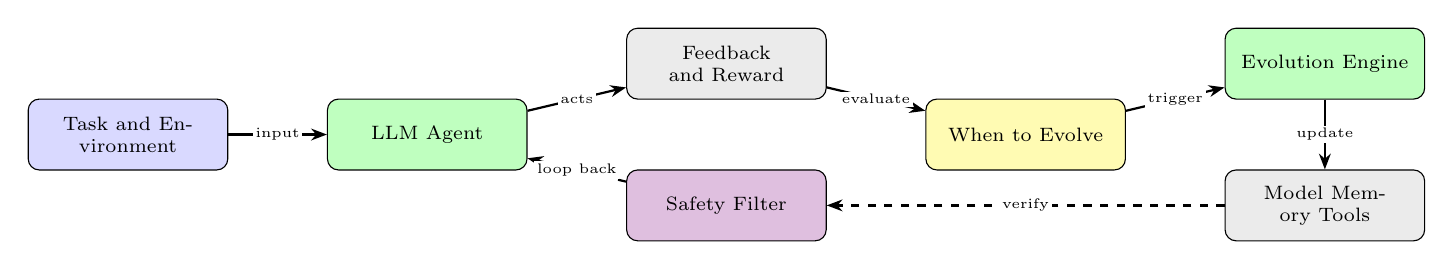
\begin{tikzpicture}
    \node[kuser] (task) at (0.00,0.00) {Task and Environment};
    \node[kagent] (agent) at (3.80,0.00) {LLM Agent};
    \node[kdata] (feedback) at (7.60,0.90) {Feedback and Reward};
    \node[kguard] (guard) at (7.60,-0.90) {Safety Filter};
    \node[kdecision] (when) at (11.40,0.00) {When to Evolve};
    \node[kagent] (engine) at (15.20,0.90) {Evolution Engine};
    \node[kdata] (what) at (15.20,-0.90) {Model Memory Tools};
    \draw[flow] (task) -- (agent) node[midway, font=\tiny, fill=white, inner sep=1pt]{input};
    \draw[flow] (agent) -- (feedback) node[midway, font=\tiny, fill=white, inner sep=1pt]{acts};
    \draw[flow] (feedback) -- (when) node[midway, font=\tiny, fill=white, inner sep=1pt]{evaluate};
    \draw[flow] (when) -- (engine) node[midway, font=\tiny, fill=white, inner sep=1pt]{trigger};
    \draw[flow] (engine) -- (what) node[midway, font=\tiny, fill=white, inner sep=1pt]{update};
    \draw[flow, dashed] (what) -- (guard) node[midway, font=\tiny, fill=white, inner sep=1pt]{verify};
    \draw[flow, dashed] (guard) -- (agent) node[midway, font=\tiny, fill=white, inner sep=1pt]{loop back};
  \end{tikzpicture}%
  }
  \end{center}
  \begin{center}\scriptsize The self-evolution loop: an agent acts, gathers feedback, updates its model, memory, or tools, and applies the change through a safety check.\end{center}
\end{frame}
\note{This diagram shows the self-evolution loop. On the left, a task comes in from the environment, whether that is coding, education, or healthcare. The agent acts and gets feedback or a reward. That feedback triggers a decision about when to evolve, an evolution engine updates the model, memory, or tools, and a safety filter checks the change before it loops back into a smarter agent.}
\begin{frame}[allowframebreaks]{How It Works (Explained)}
\begin{itemize}
  \item Left: a task from the environment (coding, education, healthcare) enters the agent.
  \item The LLM agent acts, using its tools and memory to attempt the task.
  \item Its actions produce feedback and rewards that measure how well it did.
  \item A when-to-evolve decision triggers learning during or between tasks.
  \item The evolution engine (how) updates the model, memory, or tools.
  \item A safety filter verifies the update before it loops back into a smarter agent.
\end{itemize}
\end{frame}
\section{Example Walkthrough}
\begin{frame}[allowframebreaks]{Example Walkthrough: A Coding Agent That Learns From Its Bugs}
\begin{enumerate}
  \item A user asks the agent to fix a failing software bug.
  \item The agent writes a patch and runs the project's tests.
  \item Tests fail, giving concrete feedback about which checks broke.
  \item The agent reflects in words: my fix missed a null case.
  \item It stores this lesson in memory and rewrites the patch.
  \item Tests now pass, and the saved lesson helps on similar future bugs.
  \item Over many tasks, the agent's success rate steadily improves.
\end{enumerate}
\end{frame}
\note{Let's make it concrete with a coding agent. A user asks it to fix a bug, so it writes a patch and runs the tests. The tests fail, which is actually useful feedback, and the agent reflects in plain language that it missed a null case. It saves that lesson to memory, fixes the patch, and next time a similar bug shows up it already knows what to check.}
\section{Results}
\begin{frame}[allowframebreaks]{Results / Findings}
\begin{itemize}
  \item First comprehensive survey dedicated entirely to self-evolving agents.
  \item Organizes the field with a four-axis taxonomy: what, when, how, where.
  \item Defines three optimization paradigms: in-context, reinforcement, gradient-based.
  \item Proposes five evaluation goals: adaptivity, retention, generalization, efficiency, safety.
  \item Spans 77 pages with 9 figures, synthesizing hundreds of papers.
  \item Spotlights three flagship domains: coding, education, and healthcare.
\end{itemize}
\end{frame}
\note{So what does the survey actually deliver? It is the first comprehensive map of this area, built around that four-part taxonomy. It names three ways agents evolve and five things we should measure, like adaptivity and safety. It is a big piece of work, around 77 pages with 9 figures, pulling together hundreds of papers, and it spotlights coding, education, and healthcare.}
\section{Discussion}
\begin{frame}{Discussion}
\begin{itemize}
  \item Self-evolution shifts agents from static tools to lifelong learners.
  \item Textual feedback loops (Reflexion-style) enable learning without costly retraining.
  \item Multi-agent co-evolution can improve faster than single-agent self-improvement.
  \item A shared taxonomy lets researchers compare otherwise scattered methods.
\end{itemize}
\end{frame}
\note{The big takeaway is a shift in mindset, from agents as fixed tools to agents as lifelong learners. Interestingly, a lot of the progress comes from simple language feedback loops rather than expensive retraining. And when several agents evolve together, they can often improve faster than one agent working alone.}
\section{Challenges}
\begin{frame}{Limitations \& Challenges}
\begin{itemize}
  \item Evolving agents risk catastrophic forgetting of earlier skills.
  \item Open-ended self-improvement is hard to evaluate reliably.
  \item As a survey, it maps methods but runs no new experiments.
  \item Safe, aligned self-modification remains largely unsolved.
\end{itemize}
\end{frame}
\note{A few honest caveats. These agents can forget old skills while learning new ones, and open-ended self-improvement is genuinely hard to measure. Remember this is a survey, so it maps the landscape rather than running new experiments. And making self-modification safe is still very much an open problem.}
\section{Future Work}
\begin{frame}{Future Work}
\begin{itemize}
  \item Build standard benchmarks that measure long-term adaptation.
  \item Develop safety guards for autonomous self-modification.
  \item Study co-evolution among many interacting agents.
  \item Improve efficiency so evolution scales to large models.
\end{itemize}
\end{frame}
\note{Looking ahead, the authors call for better benchmarks that test learning over the long haul, and stronger safety guards for agents that change themselves. They are also excited about many agents co-evolving together, and about making all of this efficient enough to work on large models.}
\section{Conclusion}
\begin{frame}{Conclusion}
\begin{itemize}
  \item Static LLM agents cannot keep up with changing tasks.
  \item Self-evolving agents learn continually from feedback and experience.
  \item The what-when-how-where framework organizes this emerging field.
  \item Safety and evaluation are the key hurdles on the path ahead.
\end{itemize}
\end{frame}
\note{To wrap up: static agents just cannot keep pace with a changing world, and self-evolving agents offer a path forward by learning continually from feedback. The what, when, how, and where framework gives us a clean way to think about the field. The two things to keep watching are safety and evaluation.}
\section{References}
\begin{frame}[allowframebreaks]{References}
  \footnotesize
  \begin{enumerate}
    \item Gao, H.-a., Geng, J., Hua, W., Hu, M., et al. (2025). A Survey of Self-Evolving Agents: What, When, How, and Where to Evolve on the Path to Artificial Super Intelligence. arXiv:2507.21046. Transactions on Machine Learning Research (2026).
    \item Shinn, N., Cassano, F., Gopinath, A., Narasimhan, K., Yao, S. (2023). Reflexion: Language Agents with Verbal Reinforcement Learning. NeurIPS 2023. arXiv:2303.11366.
    \item Wang, G., Xie, Y., Jiang, Y., et al. (2023). Voyager: An Open-Ended Embodied Agent with Large Language Models. arXiv:2305.16291.
    \item Madaan, A., Tandon, N., Gupta, P., et al. (2023). Self-Refine: Iterative Refinement with Self-Feedback. NeurIPS 2023. arXiv:2303.17651.
    \item Yao, S., Zhao, J., Yu, D., et al. (2023). ReAct: Synergizing Reasoning and Acting in Language Models. ICLR 2023. arXiv:2210.03629.
    \item Yuan, W., Pang, R. Y., Cho, K., et al. (2024). Self-Rewarding Language Models. arXiv:2401.10020.
  \end{enumerate}
\end{frame}
\begin{frame}[plain]
  \begin{center}
    {\Huge Thank You}\\[1em]
    {\large Questions?}
  \end{center}
\end{frame}
\end{document}